\documentclass[12pt]{scrartcl}
\usepackage{ucs}
\usepackage[utf8x]{inputenc}
\usepackage[T1]{fontenc}
\usepackage[ngerman]{babel}
\usepackage{graphicx}
\usepackage{float}
\usepackage{listings}
\usepackage[table,xcdraw]{xcolor}
\usepackage[automark]{scrpage2}
\usepackage[normalem]{ulem}
\usepackage{listings}
\useunder{\uline}{\ul}{}
\pagestyle{scrheadings}
\clearscrheadfoot
\ifoot[]{\author}
\ofoot[]{\pagemark}
\lstset{basicstyle=\ttfamily,
showstringspaces=false,
commentstyle=\color{red},
keywordstyle=\color{blue},
breaklines=true,
literate=%
{Ö}{{\"O}}1
{Ä}{{\"A}}1
{Ü}{{\"U}}1
{ß}{{\ss}}2
{ü}{{\"u}}1
{ä}{{\"a}}1
{ö}{{\"o}}1
}

%\title{Modul zum Import verschiedener Dateiformate}
%\author{Mark Unger und Siegfried Kienzle}
%\date{Konstanz, den \today{}}



\begin{document}

\begin{titlepage}
	\centering
	
\includegraphics[width=0.5\textwidth]{HTWG}\par\vspace{2.5cm}
	\vspace{1cm}
	{\scshape\Large Handbuch für\par}
	\vspace{1.5cm} 
	{\scshape\bfseries Modul zum Import verschiedener Dateiformate\par}
	\vspace{2cm}
	{\Large\itshape Mark Unger und Siegfried Kienzle\par}
	\vfill

% Bottom of the page
	{\large \today\par}
\end{titlepage}


\newpage

\begin{center}
\section*{Erklärung}
Die in diesem Projekt verwendete Software unterliegt den 
rechtlich jeweiligen Bestimmungen der einzelnen Organisationen und Firmen. 
\vfill
\end{center}

\newpage
\tableofcontents
\newpage

\section{Modul}
\label{sec:modul-einleitung}

\subsection{Über die Software}
\label{sec:software-einleitung}
Dieses Modul dient zur Extrahierung von Text aus Dateien. 
Sie können dieses Modul für folgende Endungen verwenden:
\begin{itemize}
	\item .doc
	\item .docx
	\item .odt
	\item .pdf
	\item rtf
\end{itemize}
Es wurde für Python 3.4.3 entwickelt und unter 
Ubuntu 14.04.05 LTS getestet. Zur Installation liegt 
ein Bash-Script vor. 

\subsection{Über das Handbuch}
\label{sec:handbuch-einleitung}
Dieses Handbuch beschreibt die Installation und die Handhabung
mit dem Modul. 


\newpage
\section{Grundlagen}
\label{sec:grundlagen}
\subsection{Installation}
\label{sec:grundlagen-installation}
\begin{enumerate}

\item Installationsscript mittels ./inst.sh aufrufen:
\newline
\begin{figure}[htbp]
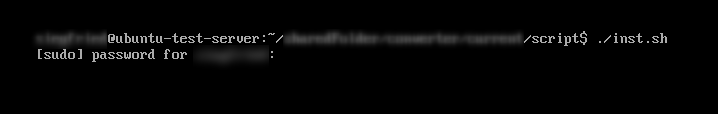
\includegraphics[width=1.0\textwidth]{schritt1}\par\vspace{0.5cm}
\caption{Nach Aufruf des Installationscriptes ./inst.sh}
\label{fig:script1}
\end{figure}
\item sudo-Passwort eintippen und die Enter-Taste drücken.
\item Es werden nun einige Abhängigkeiten installiert, die 
zur Ausführung dieses Moduls benötigt werden.
\newpage
\item Geben Sie nun den Pfad an, in den das Modul installiert werden soll.
Sollte der Pfad nicht existieren, werden Sie wie in Abbildung 4 gefragt
ob der Pfad erstellt werden soll. 
Existiert der Pfad, entfallen die Schritte 6 bis 8. 
\begin{figure}[htbp]
\centering
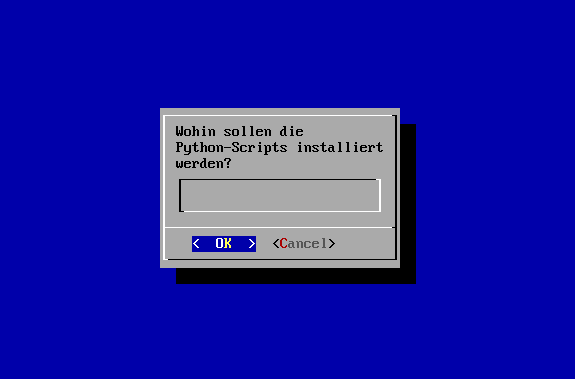
\includegraphics[width=0.6\textwidth]{schritt2}\par\vspace{0.5cm}
\caption{Nach Aufruf des Installationscriptes ./inst.sh}
\label{fig:script2}
\end{figure}
\begin{figure}[htbp]
\centering
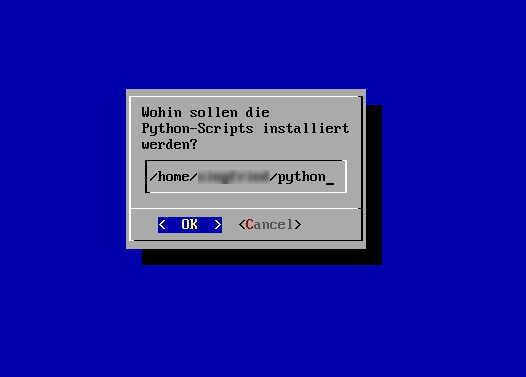
\includegraphics[width=0.6\textwidth]{schritt3}\par\vspace{0.5cm}
\caption{Nach Eingabe des Installationspfads}
\label{fig:script3}
\end{figure}
\item Wenn der OK-Button blau hinterlegt ist, können Sie mit
der Enter-Taste den Pfad bestätigen. 
\newpage
\item Sollte kein Pfad existieren, erscheint folgendes Fenster:
\begin{figure}[htbp]
\centering
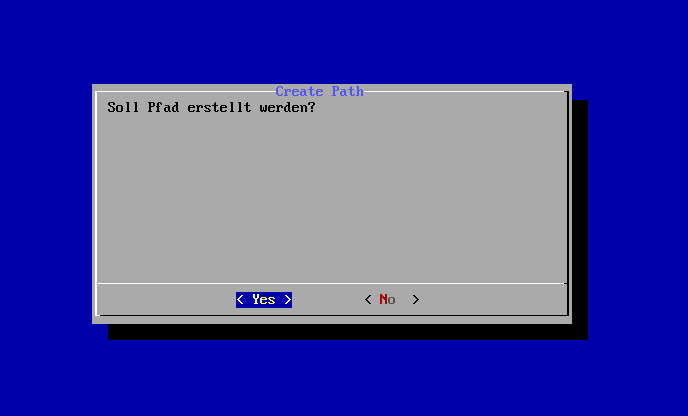
\includegraphics[width=1.0\textwidth]{schritt4}\par\vspace{0.5cm}
\caption{Pfad erstellen?}
\label{fig:script4}
\end{figure}
\item Wählen Sie nun mit den Pfeiltasten aus, ob Sie den Pfad erstellen möchten
oder nicht und drücken Sie dann die Enter-Taste.
\begin{figure}[htbp]
\centering
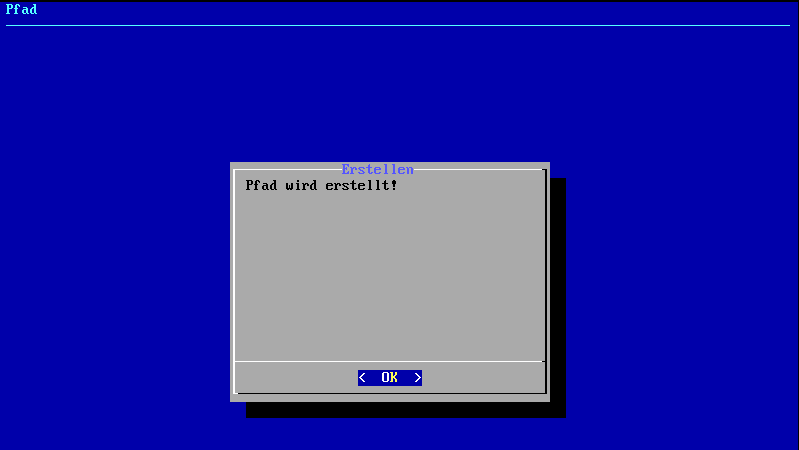
\includegraphics[width=0.8\textwidth]{schritt5}\par\vspace{0.5cm}
\caption{Pfad wurde erstellt}
\label{fig:script5}
\end{figure}
\newpage
\item Es wurde nun der Pfad erstellt. Drücken Sie nun die Enter-Taste, um die Dateien
in das entsprechend vorher erstellte Verzeichnis, zu entpacken.
\begin{figure}[htbp]
\centering
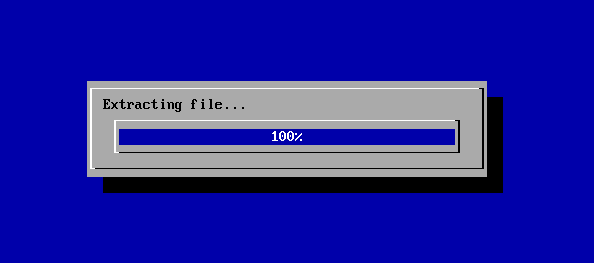
\includegraphics[width=0.8\textwidth]{schritt6}\par\vspace{0.5cm}
\caption{Pfad wurde erstellt}
\label{fig:script6}
\end{figure}
\item Die Installation ist nun abgeschlossen. Prüfen Sie nun 
bitte ob alle Dateien installiert wurden. Eine genaue Auflistung finden
Sie unter dem Punkt 2.3.
\end{enumerate} 
\subsection{Bestandteile Installationspaket}
\label{sec:installationsbestandteile}
\begin{table}[H]
\centering
\label{installationsbestandteile}
\begin{tabular}{|l|l|}
\hline
\rowcolor[HTML]{9B9B9B} 
Datei      & Beschreibung                                                      \\ \hline
inst.sh    & Bash-Script für die Ausführung als Super-User (sudo) unter Ubuntu \\ \hline
ubuntu.sh  & Bash-Script für die Installation unter Ubuntu                     \\ \hline
moduls.tar & Tar-Datei, die die Python-Module enthält                          \\ \hline
\end{tabular}
\caption{Bestandteile Installationspaket}
\end{table}
\subsection{Modulbestandteile}
\label{sec:modulbestandteile}
\begin{table}[H]
\centering
\label{modulbestandteil}
\begin{tabular}{|l|l|}
\hline
\rowcolor[HTML]{9B9B9B} 
Datei           & Verwendung                           \\ \hline
convertToTxt.py & Datei die für das Extrahieren aufgerufen wird \\ \hline
extractTxt.py   & Hauptdatei für die Extrahierung      \\ \hline
loggingModule.py           & Hilfsdatei die Fehler in Logging-Datei schreibt        \\ \hline
docTxt.py       & Modul für die Dateiendung doc        \\ \hline
docxTxt.py      & Modul für die Dateiendung docx       \\ \hline
odtTxt.py       & Modul für die Dateiendung odt        \\ \hline
pdfTxt.py       & Modul für die Dateiendung pdf        \\ \hline
rtfTxt.py       & Modul für die Dateiendung rtf        \\ \hline
\end{tabular}
\caption{Modulbestandteile}
\end{table}
\newpage
\subsection{Erste Schritte}
\label{sec:first-steps}
\subsubsection{Genereller Aufruf}
\label{sec:first-steps-general}
Im Allgemeinen wird das Modul wie folgt aufgerufen:
%ersteSchritte001
\begin{figure}[htbp]
\centering
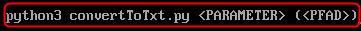
\includegraphics[width=0.7\textwidth]{ersteSchritte001}\par\vspace{0.25cm}
%\caption{Aufruf der Hilfe mittels -h}
\label{fig:ersteSchritteGeneral001}
\end{figure}
\newline
Dabei sollte <PARAMETER> durch Parameter aus Tabelle 3 ersetzt werden. Bei  den Parametern -p bzw. -{}-process sowie bei -o bzw. -{}-output sollte dann zusätzlich <PFAD> (das hier in runden Klammern steht) durch den Pfad der Datei, aus der der Text extrahiert werden soll, ersetzt werden. 
Außerdem ist zwingend darauf zu achten, dass das Modul mit python3 aufgerufen wird.
\begin{table}[H]
\begin{center}
\label{params}
\begin{tabular}{|l|l|l|}
\hline
\rowcolor[HTML]{C0C0C0} 
Parameter (kurz) & Parameter (lang) & Erklärung                                                                                                                              \\ \hline
-h               & -{}-help           & Zeigt die Hilfe an                                                                                                                     \\ \hline
-p               & -{}-process        & Führt die Textextrahierung durch.  \\ \hline
-v				 & ------------------ & Verbose-Mode: Gibt den Text auf Konsole aus. \\ \hline
-o               & -{}-output         & Parameter für die Ausgabedatei.\\
				 &					  &	Nur anwendbar mit Argument -p bzw. -{}-process \\ \hline
\end{tabular}
\caption{Parameterübersicht}
\end{center}
\end{table}

Beispielaufrufe finden Sie weiter unten in diesem Kapitel. 
\newpage
\subsubsection{Extrahieren von Text auf Konsole}
\label{sec:first-steps-extraction-console}
Zum Extrahieren von Text tippen Sie einfach	

\begin{lstlisting}[language=bash]
python3 convertToTxt.py -p <DATEIPFAD> -v 
\end{lstlisting}\begin{center}
oder 
\end{center}
\begin{lstlisting}[language=bash]
python3 convertToTxt.py --process <DATEIPFAD> -v
\end{lstlisting}
Als Beispiel sehen Sie im folgenden wie Text aus einer DOCX-Datei extrahiert wird:
\begin{figure}[htbp]
\centering
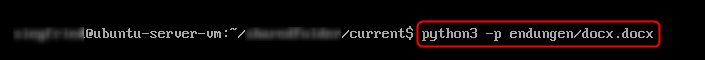
\includegraphics[width=0.7\textwidth]{ersteSchritteExtract001}\par\vspace{0.25cm}
%\caption{Aufruf der Hilfe mittels -h}
\label{fig:ersteSchritteExtract001}
\end{figure}
\begin{center}
oder
\end{center}
\begin{figure}[htbp]
\centering

\includegraphics[width=0.7\textwidth]{ersteSchritteExtract002}\par\vspace{0.25cm}
%\caption{Aufruf der Hilfe mittels -h}
\label{fig:ersteSchritteExtract002}
\end{figure}
\begin{figure}[htbp]
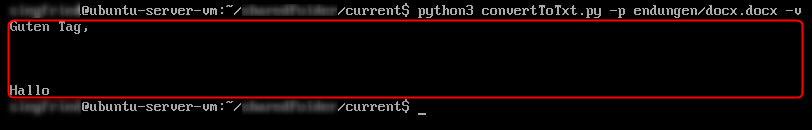
\includegraphics[width=1.0\textwidth]{ersteSchritteExtract003}\par\vspace{0.25cm}
\caption{Beispielausgabe von docx}
\label{fig:ersteSchritteExtract003}
\end{figure}
\newpage
\subsubsection{Extrahieren von Text in eine Datei ohne Konsolenausgabe}
\label{sec:first-steps-extraction-file-without}
Zum Extrahieren von Text in eine Datei, ohne dabei den Text auf die Konsole auszugeben, tippen Sie einfach 
\begin{lstlisting}[language=bash]
python3 convertToTxt.py -p <DATEIPFAD> -o <AUSGABEDATEI>
\end{lstlisting}
\begin{center}
oder
\end{center}
\begin{lstlisting}[language=bash]
python3 convertToTxt.py --process <DATEIPFAD> --output <AUSGABEDATEI>
\end{lstlisting} 
Es ist zu beachten, dass wenn die angegebene Ausgabedatei bereits existiert, der Inhalt durch den Text der im Moment extrahiert wird, überschrieben wird. 
Als Beispiel sehen Sie im folgenden wie Text aus einer DOCX-Datei extrahiert wird:
\begin{figure}[htbp]
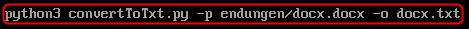
\includegraphics[width=1.0\textwidth]{ersteSchritteExtractIntoFileWithoutConsole001}\par\vspace{0.25cm}
%\caption{Aufruf der Hilfe mittels -h}
\label{fig:ersteSchritteExtractIntoFileWithoutConsole001}
\end{figure}
\begin{center}
oder
\end{center}
\begin{figure}[htbp]
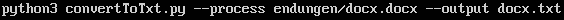
\includegraphics[width=1.0\textwidth]{ersteSchritteExtractIntoFileWithoutConsole002}\par

\vspace{0.25cm}
%\caption{Aufruf der Hilfe mittels -h}
\label{fig:ersteSchritteExtractIntoFileWithoutConsole002}
\end{figure}
\begin{figure}[htbp]
\centering
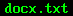
\includegraphics[width=0.2\textwidth]{ersteSchritteExtractIntoFileWithoutConsole003}\par\vspace{0.25cm}
\caption{Beispielausgabe des Befehls ls, nachdem die Datei erstellt wurde}
\label{fig:ersteSchritteExtractIntoFileWithoutConsole003}
\end{figure}
\newpage
\subsubsection{Extrahieren von Text in eine Datei mit Konsolenausgabe}
\label{sec:first-steps-extraction-file-with}
Zum Extrahieren von Text in eine Datei mit Konsolenausgabe, tippen Sie einfach 
\begin{lstlisting}[language=bash]
python3 convertToTxt.py -p <DATEIPFAD> -o <AUSGABEDATEI> -v
\end{lstlisting}
\begin{center}
oder
\end{center}
\begin{lstlisting}[language=bash] 
python3 convertToTxt.py --process <DATEIPFAD> --output <AUSGABEDATEI> -v
\end{lstlisting}
Es ist zu beachten, dass wenn die angegebene Ausgabedatei bereits existiert, der Inhalt durch den Text der im Moment extrahiert wird, überschrieben wird.
 Als Beispiel sehen Sie im folgenden wie Text aus einer DOCX-Datei extrahiert wird:
\begin{figure}[htbp]

\includegraphics[width=1.0\textwidth]{ersteSchritteExtractIntoFileWithConsole001}\par\vspace{0.25cm}
%\caption{Aufruf der Hilfe mittels -h}
\label{fig:ersteSchritteExtractIntoFileWithConsole001}
\end{figure}
\begin{center}
oder
\end{center}
\begin{figure}[htbp]

\includegraphics[width=1.0\textwidth]{ersteSchritteExtractIntoFileWithConsole002}\par

\vspace{0.25cm}
%\caption{Aufruf der Hilfe mittels -h}
\label{fig:ersteSchritteExtractIntoFileWithConsole002}
\end{figure}
\begin{figure}[htbp]
\centering
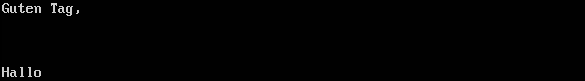
\includegraphics[width=1.0\textwidth]{ersteSchritteExtractIntoFileWithConsole003}\par\vspace{0.25cm}
\caption{Ausgabe nach Aufruf des obigen Befehls}
%\label{fig:ersteSchritteExtractIntoFileWithoutConsole003}
\end{figure}
\newpage
\subsubsection{Hilfe aufrufen}
\label{sec:first-steps-help}
Zum Aufrufen der Hilfe einfach wie im folgenden Bild den Parameter -h bzw. -{}-help eingeben.
\newline
\begin{figure}[htbp]
\centering
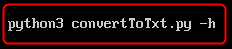
\includegraphics[width=0.4\textwidth]{ersteSchritteHilfe1}\par\vspace{0.25cm}
%\caption{Aufruf der Hilfe mittels -h}
\label{fig:ersteSchritteHilfe1}
\end{figure}
\begin{center}
oder
\end{center}
\begin{figure}[htbp]
\centering
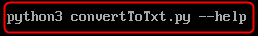
\includegraphics[width=0.4\textwidth]{ersteSchritteHilfe2}\par\vspace{0.25cm}
%\caption{Aufruf der Hilfe mittels - -help}
\label{fig:ersteSchritte2}
\end{figure}
Die Ausgabe sollte wie folgt aussehen:
\begin{figure}[htbp]
\centering
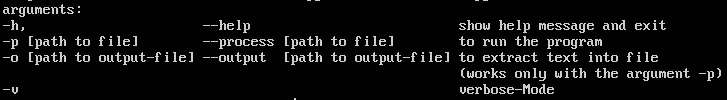
\includegraphics[width=1.1\textwidth]{ersteSchritteHilfe3}\par\vspace{0.5cm}
%\caption{Aufruf der Hilfe mittels - -help}
\label{fig:ersteSchritteHilfe3}
\end{figure}
\newpage
\section{Technischer Hintergrund}
\label{sec:technical-background}
\subsection{Verwendete Fremdsoftware}
\label{sec:technical-background-additional-software}
\begin{table}[H]
\centering

\label{additional-software-table}
\begin{tabular}{|l|l|l|}
\hline
\rowcolor[HTML]{C0C0C0} 
Datiename  & verwendete Zusatzsoftware & {\color[HTML]{000000} Entwicklerwebseite}     \\ \hline
docTxt.py  & catdoc                    & http://freecode.com/projects/catdoc           \\ \hline
docxTxt.py & Python-Modul docx2txt     & http://docx2txt.sourceforge.net/              \\ \hline
pdfTxt.py  & pdftotext                 & https://poppler.freedesktop.org/              \\ \hline
odtTxt.py  & odt2txt                   & https://github.com/dstosberg/odt2txt          \\ \hline
rtfTxt.py  & unrtf                     & https://www.gnu.org/software/unrtf/unrtf.html \\ \hline
\end{tabular}
\caption{Auflistung der verwendeten Software}
\end{table}
\subsection{Aufbau}
\label{sec:technical-background-aufbau}
Wie schon aus der Tabelle in Kapitel \ref{modulbestandteil} zu sehen ist, besteht das Projekt aus einer Hauptdatei convertToTxt.py die aufgerufen wird, einer Hilfsdatei extractTxt.py in die die Programmlogik ausgelagert wurde und den einzelnen Modulen.
Im weiteren werden die einzelnen Dateien technisch erläutert.
\subsubsection{convertToTxt.py}
\label{sec:technical-background-convertToTxt}
Die convertToTxt.py nimmt alle Anfragen entgegen und beinhaltet die einzelnen Argumente sowie die Hilfe-Funktion.
Die Verarbeitung der Argumente und Optionen wurden mittels dem Modul getopt realisert.
\subsubsection{extractTxt.py}
\label{sec:technical-background-extractTxt}
Die Datei extractTxt.py enthält die eigentliche Logik des Extrahierungs-Skriptes. Sie enthält die Funktionen process(path) und file(text, a).
Die process(path)-Funktion nimmt den Pfad aus der zu extrahierenden Datei über den Parameter path entgegen und übergibt den Pfad dem entsprechenden Modul, indem es sich die Dateiendung betrachtet. 
Der heraus zu extrahierende Text, der von einzelnen Modulen zurückgegeben wird, wird mit UTF-8 dekodiert und so dann endgültig zurückgegeben. 
file(text, a) speichert den heraus extrahierten Text in eine Datei. Dazu wird dem Parameter text der zu speichernde Text und dem Parameter a der Speicherort übergeben. 
\subsubsection{Die Module}
\label{sec:technical-background-module}
Wie im Abschnitt \ref{additional-software-table} in der Tabelle zu sehen ist, gibt es fünf Module. Alle Module rufen, bis auf docxTxt.py, ein Konsolen-Programm mittels subprocess.Popen() auf.
Es wird dazu das Modul subprocess importiert. In einer Liste, die dem subprocess.Popen() übergeben wird, steht das zu ausführende Programm und der Dateiname. Außerdem wird die Standardausgabe und die Ausgabe für die Fehler in eine Pipe umgeleitet, damit der zu extrahierte Text später weiterverarbeitet werden kann. Am Ende wird dann process.stdout.read() zurückgeliefert und mit process.stdout.close(), wird der Lese-Stream dann wieder geschlossen.
Die Fehlerbehandlung wurde mittels try-except-Anweisung realisiert und es wird bei einer auftretenden Exception in ein Logfile namens logging.log geschrieben. Das komplette Logging wurde in die Datei loggingModule.py ausgelagert. 
\newline
Das Modul docxTxt.py unterscheidet sich von den anderen Modulen in sofern, dass ein Modul namens docx2txt importiert wird und dieses eigene Methoden zum Aufrufen besitzt. In docxTxt.py wird lediglich die Funktion process() verwendet. 
An die Funktion wird der Dateiname, aus der der Text extrahiert werden soll, übergeben und process() liefert dann einen String mit dem darin extrahierten Text zurück. 
\newpage
\section{Kontaktdaten}
\label{sec:kontaktdaten}
\begin{table}[H]
%\centering
\label{kontaktdaten}
\begin{tabular}{|l|l|}
\hline
\rowcolor[HTML]{9B9B9B} 
Name              & E-Mail                   \\ \hline
Mark Unger        & mrk.unger@gmail.com      \\ \hline
Siegfried Kienzle & siegfried.kienzle@gmx.de \\ \hline
\end{tabular}
%\caption{Kontaktdaten}
\end{table}
\end{document}